The timing properties, and other features measured by the timing model, for
over 2000 pulsars observed can be accessed via the ATNF pulsar catalogue
\citep{ATNF}.  We can categorise the population by their measured values of
period $P$ and period derivative $\Pdot$. This is done by plotting them in a
so-called $P - \Pdot$ diagram as shown in Fig.~\ref{fig: Period_PeriodDot}.
Some of the pulsar varieties have been marked in this plot and we now discuss
their features.

\begin{figure}[hb]
    \centering
    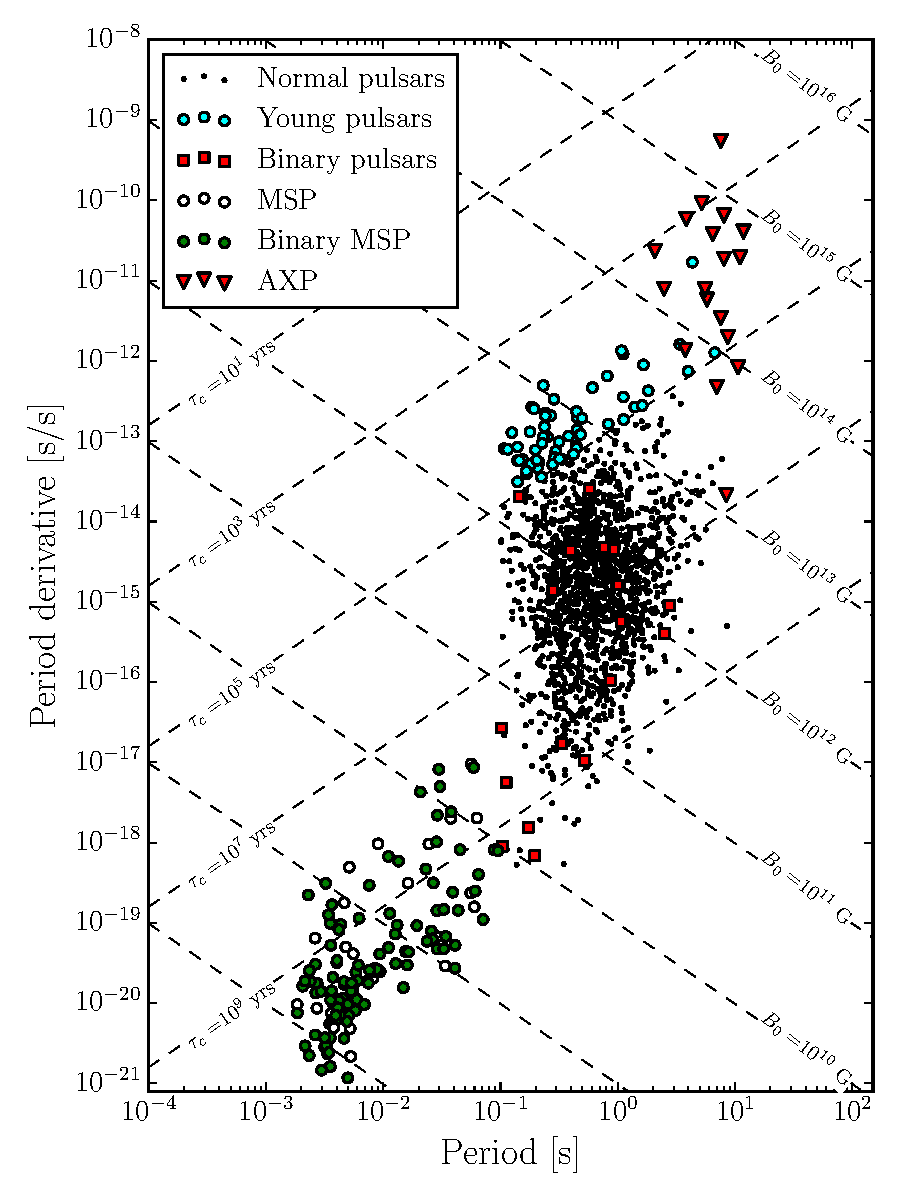
\includegraphics[width=0.8\textwidth]{Period_PeriodDot}
    \caption{Period - period diagram using data taken from the ATNF pulsar
             catalogue \citep{ATNF}. Dashed lines show inferred magnetic fields
             and characteristic ages as described in Sec.~\ref{sec: rotation
             powered pulsars}}
    \label{fig: Period_PeriodDot}
\end{figure}

The majority of pulsars, referred to as the `normal' pulsars, are
\emph{isolated} (without a binary companion) and have typical periods of
$P=10^{-1}-10^{1}$~s. These can be described as \emph{rotation powered} pulsars
since the EM radiation is powered by the loss of rotational energy. As
described later in Sec.~\ref{sec: rotation powered pulsars}, estimates can be made
for their characteristic age $\tau_{c}$ and surface magnetic field strength
$B_{0}$ based on a dipole spindown model. Constant lines of these quantities
are plotted in Fig.~\ref{fig: Period_PeriodDot}. Of the normal pulsars, we
can identify the young pulsars as those for which $\tau_{c}<10^{5}$~yrs. Some
of these, such as the Crab and Vela, can be directly associated with their
supernova remnant from which they were formed \citep{Kaspi1996}.

A second smaller population of isolated rotation powered pulsars exists with
$P<10^{-1}$~s, these are the \emph{millisecond pulsars} (MSPs). These special
class of pulsars are believed to start life as normal pulsars, but are then
spun-up through accretion from a normal star. In support of this hypothesis,
the majority of MSPs in figure \ref{fig: Period_PeriodDot} have a binary
companion \citep{wijnands1998millisecond}.  During the accretion stage, the
mechanism responsible for the electromagnetic emission is thought to switch-off
and so we do not see their pulsations. However, we can observe them in an X-ray
binary when they undergo outburst \citep{lewin1997x}; this is caused by the
heating of material in the accretion disk as the neutron star draws material
from the companion star.

Some isolated pulsars are observed as sporadic bursts of pulsed X-ray radiation,
these are known as anomalous X-ray pulsars (AXPs). The neutron stars which are
thought to produce this emission have large magnetic fields $B_{0}\gtrsim
5\times10^{13}$; as a result they are named \emph{magnetars}. The high energy
radiation is thought to result from the decay of this magnetic field.
